\pdfminorversion=4
\documentclass[aspectratio=169]{beamer}

\mode<presentation>
{
  \usetheme{default}
  \usecolortheme{default}
  \usefonttheme{default}
  \setbeamertemplate{navigation symbols}{}
  \setbeamertemplate{caption}[numbered]
  \setbeamertemplate{footline}[frame number]  % or "page number"
  \setbeamercolor{frametitle}{fg=white}
  \setbeamercolor{footline}{fg=black}
}

\usepackage[english]{babel}
\usepackage[utf8x]{inputenc}
\usepackage{tikz}
\usepackage{courier}
\usepackage{array}
\usepackage{bold-extra}
\usepackage{minted}
\usepackage[thicklines]{cancel}
\usepackage{fancyvrb}

\xdefinecolor{dianablue}{rgb}{0.18,0.24,0.31}
\xdefinecolor{darkblue}{rgb}{0.1,0.1,0.7}
\xdefinecolor{darkgreen}{rgb}{0,0.5,0}
\xdefinecolor{darkgrey}{rgb}{0.35,0.35,0.35}
\xdefinecolor{darkorange}{rgb}{0.8,0.5,0}
\xdefinecolor{darkred}{rgb}{0.7,0,0}
\definecolor{darkgreen}{rgb}{0,0.6,0}
\definecolor{mauve}{rgb}{0.58,0,0.82}

\title[2019-09-14-awkward-strangeloop]{Jagged, ragged, awkward arrays}
\author{Jim Pivarski}
\institute{Princeton University -- IRIS-HEP}
\date{September 14, 2019}

\usetikzlibrary{shapes.callouts}

\begin{document}

\logo{\pgfputat{\pgfxy(0.11, 7.4)}{\pgfbox[right,base]{\tikz{\filldraw[fill=dianablue, draw=none] (0 cm, 0 cm) rectangle (50 cm, 1 cm);}\mbox{\hspace{-8 cm}
\includegraphics[height=1 cm]{princeton-logo-long.png}\hspace{0.1 cm}\raisebox{0.1 cm}{
\includegraphics[height=0.8 cm]{iris-hep-logo-long.png}}\hspace{0.1 cm}}}}}

\begin{frame}
  \titlepage
\end{frame}

\logo{\pgfputat{\pgfxy(0.11, 7.4)}{\pgfbox[right,base]{\tikz{\filldraw[fill=dianablue, draw=none] (0 cm, 0 cm) rectangle (50 cm, 1 cm);}\mbox{\hspace{-8 cm}
\includegraphics[height=1 cm]{princeton-logo.png}\hspace{0.1 cm}\raisebox{0.1 cm}{
\includegraphics[height=0.8 cm]{iris-hep-logo.png}}\hspace{0.1 cm}}}}}

% Uncomment these lines for an automatically generated outline.
%\begin{frame}{Outline}
%  \tableofcontents
%\end{frame}

% START START START START START START START START START START START START START

% \begin{frame}{Motivation: particle physics analysis}
% \Large
% \vspace{0.23 cm}
% \begin{columns}
% \column{0.5\linewidth}
% \only<1>{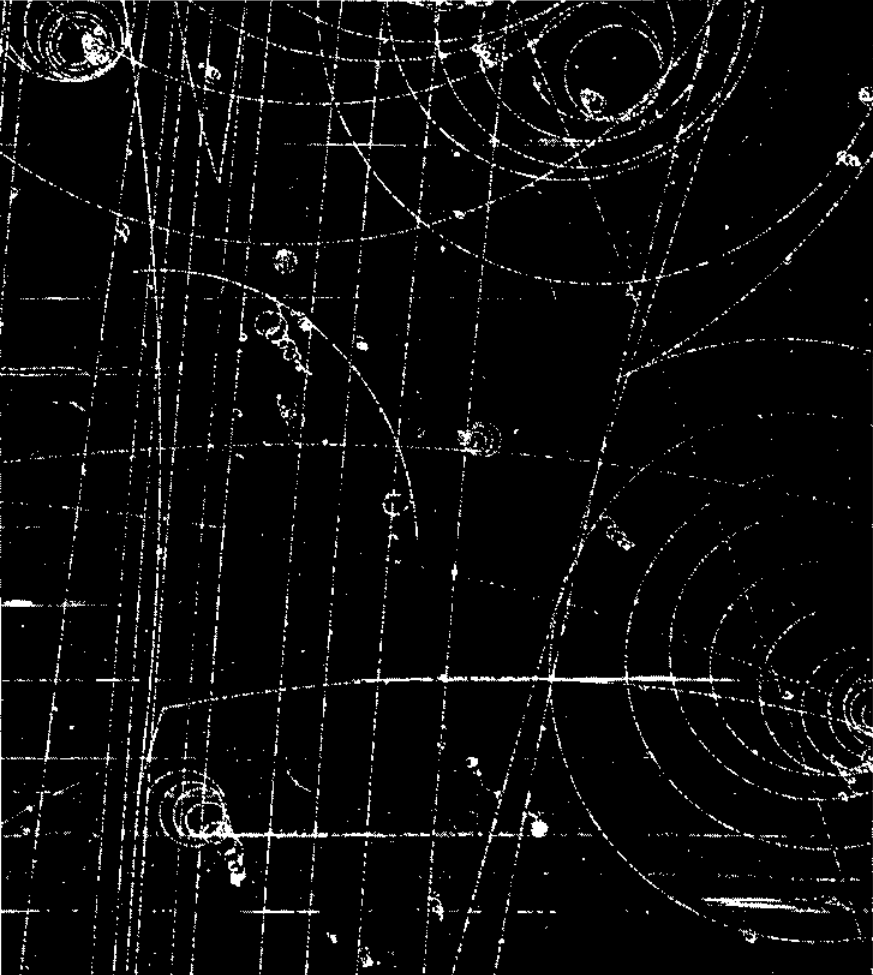
\includegraphics[width=\linewidth]{omega-minus-1.png}}\only<2->{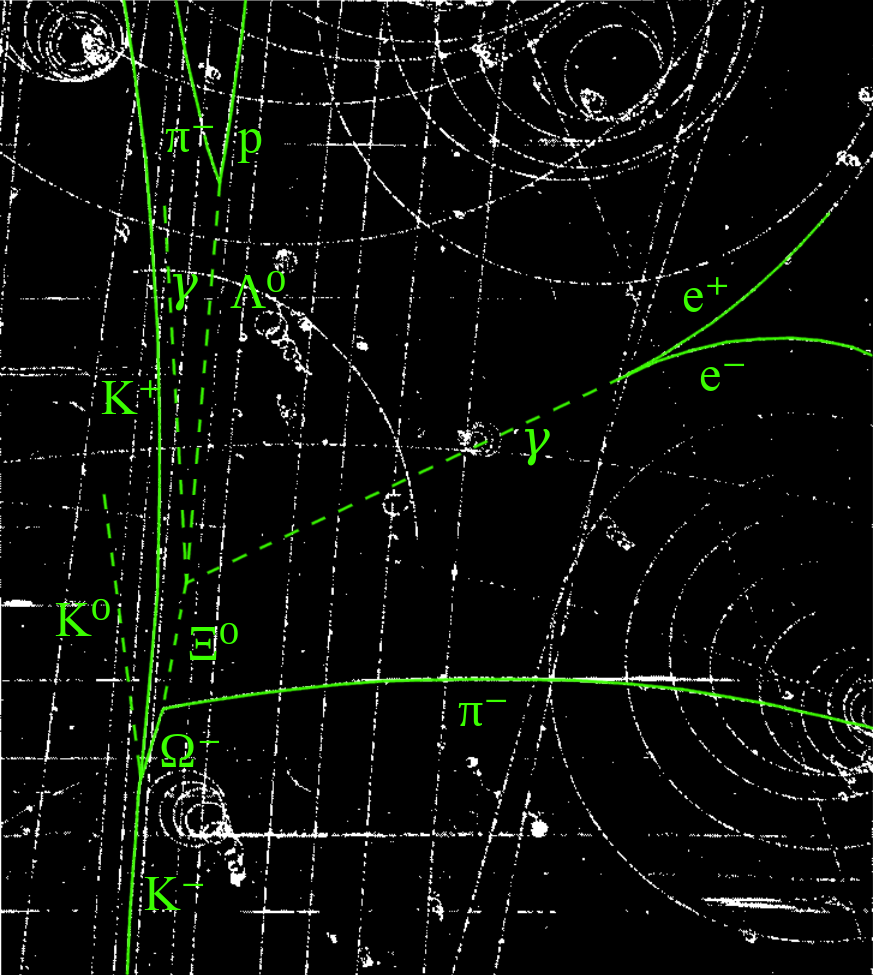
\includegraphics[width=\linewidth]{omega-minus-2.png}}
% \column{0.5\linewidth}
%
% \begin{center}
% \begin{onlyenv}<1>
% This is a famous photo: the 1964 discovery of the $\Omega$ baryon.
%
% \vspace{1 cm}
% Do you see it?
%
% \vspace{1 cm}
% \end{onlyenv}\begin{onlyenv}<2>
% How about now?
%
% \begin{align*}
% K^- + p & \to \Omega^- + K^+ + K^0 \\
% \Omega^- & \to \Xi^0 + \pi^- \\
% \Xi^0 & \to \Lambda^0 + \pi^0 \\
% \Lambda^0 & \to p + \pi^- \\
% \pi^0 & \to \gamma + \gamma
% \end{align*}
%
% \vspace{1 cm}
% \end{onlyenv}\begin{onlyenv}<3>
% This is what particle physicists do: we collide particles, produce new ones and take pictures of their decay chains.
%
% \vspace{1 cm}
% However, these pictures come to us unlabeled: lots of interactions overlap the ``interesting'' ones.
%
% \vspace{1 cm}
% \end{onlyenv}
% \end{center}
%
% \end{columns}
% \end{frame}
%
% \begin{frame}{}
% \begin{columns}
% \column{1.15\linewidth}
% 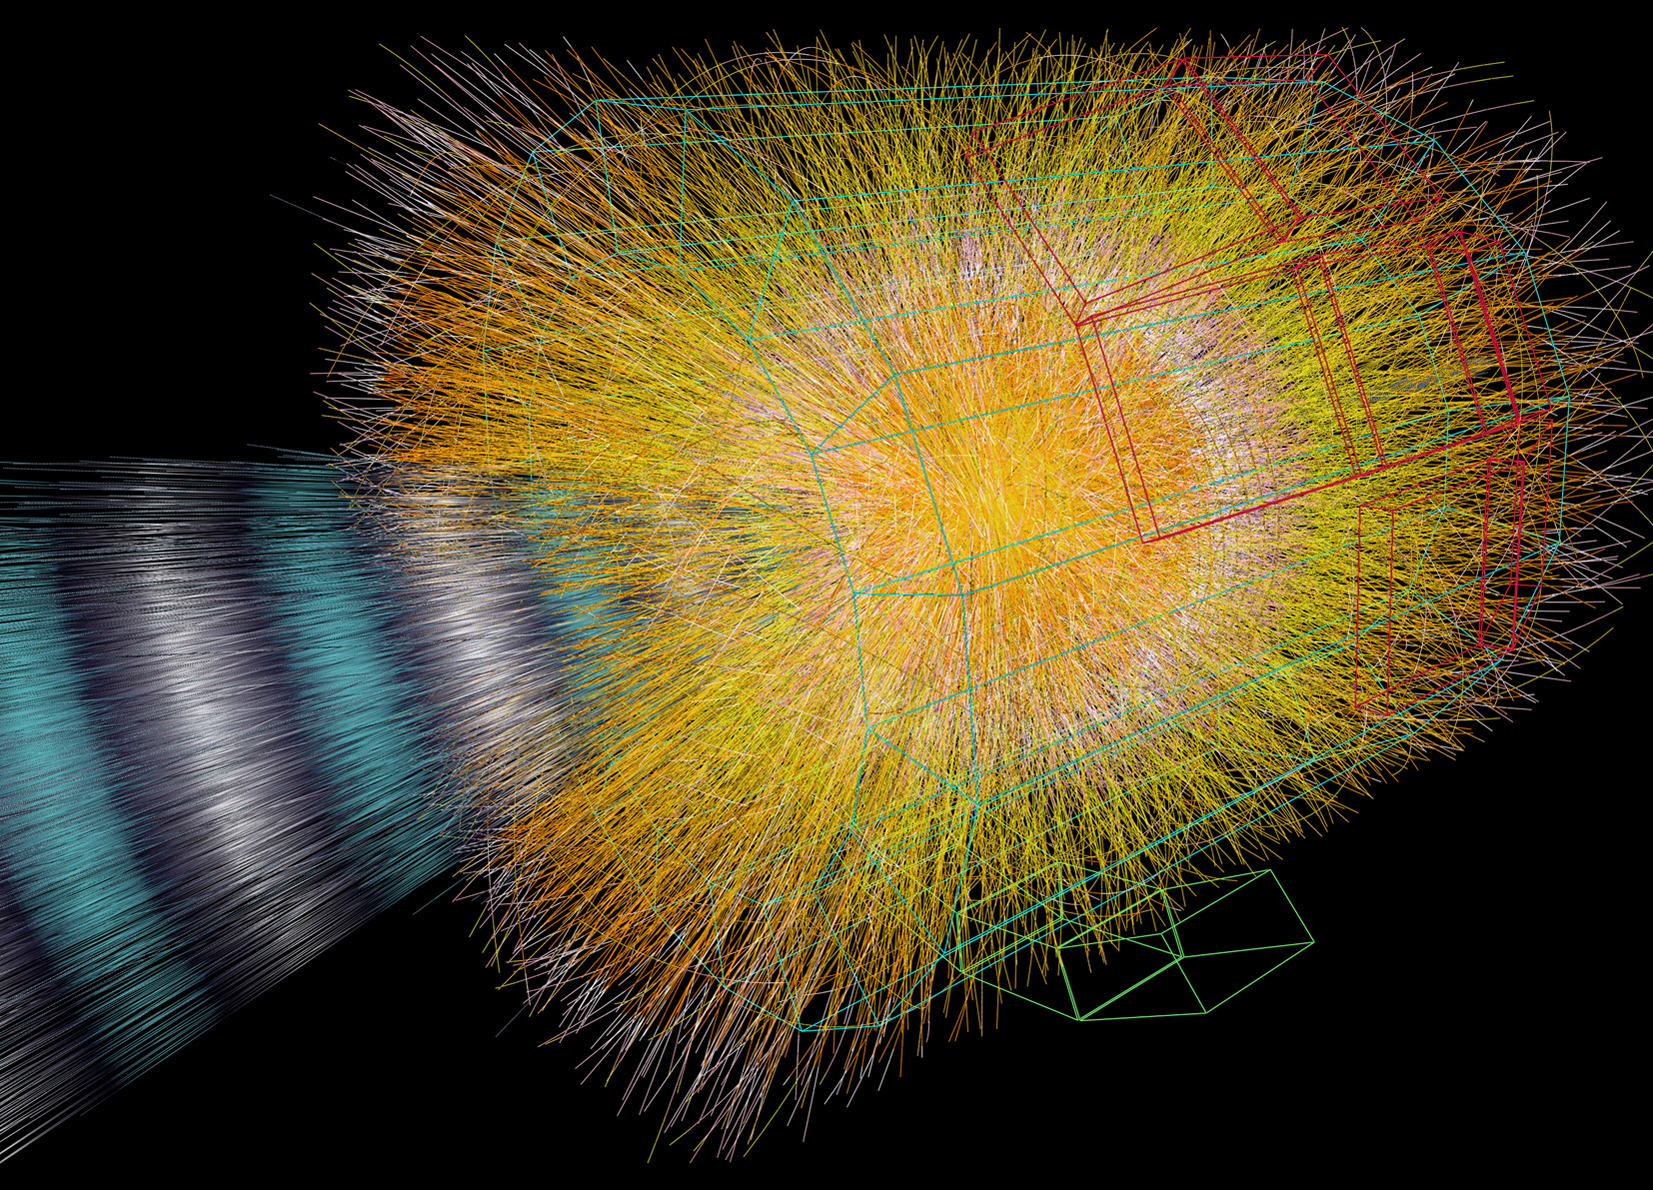
\includegraphics[width=\linewidth]{090324_ALICE-hirez.jpg}
% \end{columns}
% \end{frame}
%
% \begin{frame}{Then and now}
% \vspace{0.15 cm}
% \begin{columns}
% \column{0.32\linewidth}
% 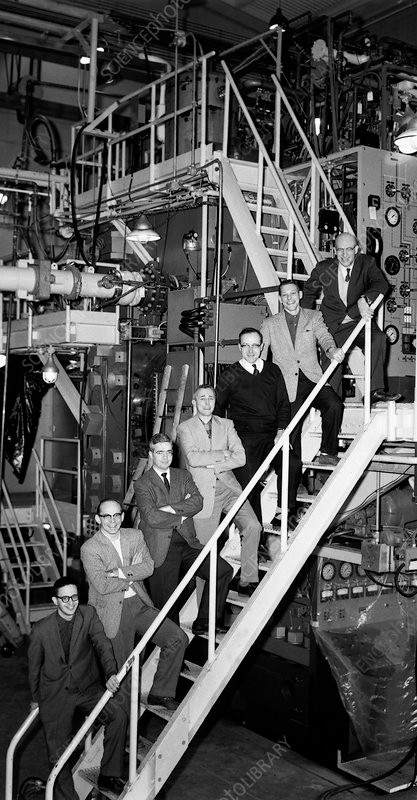
\includegraphics[width=\linewidth]{H4000010-Team_that_discovered_Omega_minus_particle.jpg}
%
% \column{0.5\linewidth}
% \begin{center}
% \begin{columns}
% \column{0.35\linewidth}
% \centering
% photographs
%
% \vspace{0.5 cm}
% 100,000 events
%
% \vspace{0.5 cm}
% manual/semi-automated scans
%
% \column{0.35\linewidth}
% \centering
% digitized signals \\
%
% \vspace{0.5 cm}
% $\sim$trillion events \\
%
% \vspace{0.5 cm}
% algorithmic searches and machine learning
% \end{columns}
% \end{center}
%
% \column{0.32\linewidth}
% 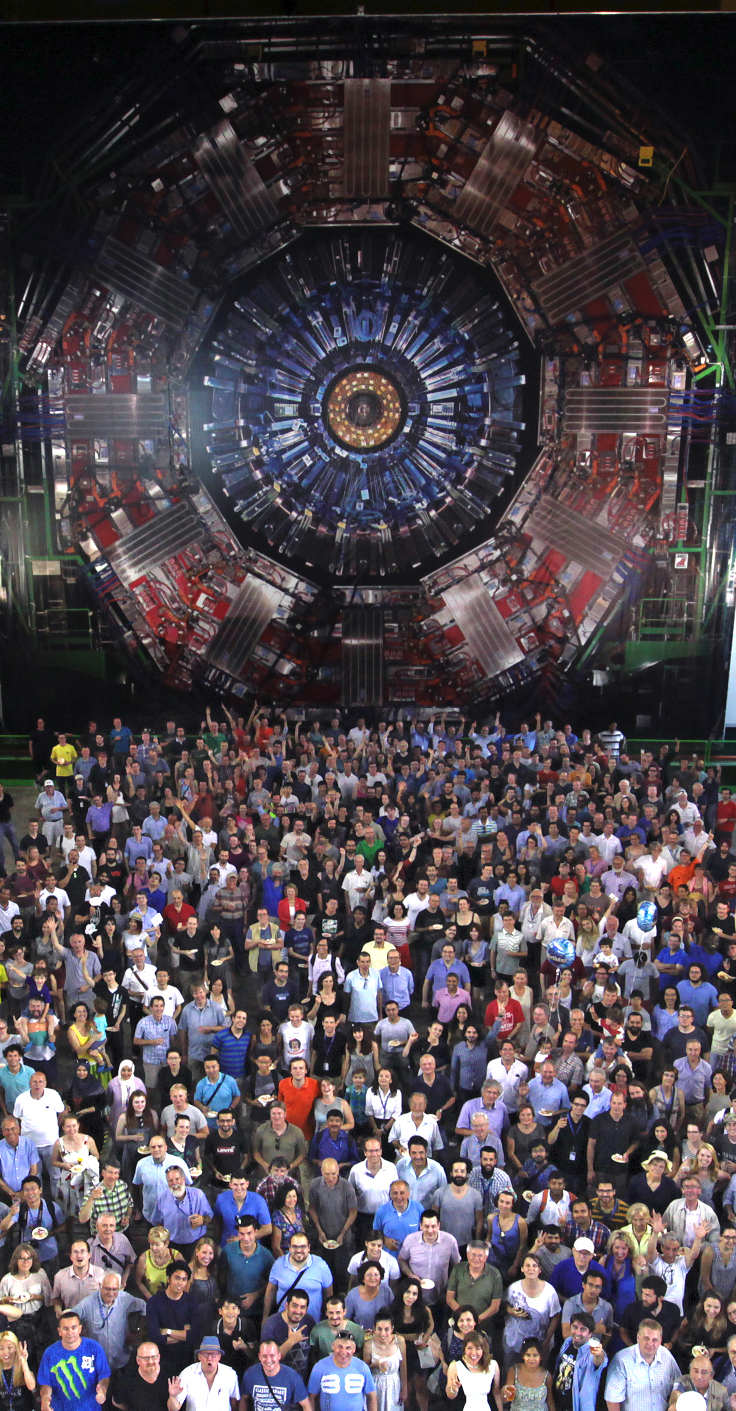
\includegraphics[width=\linewidth]{cms25_2.jpg}
% \end{columns}
% \end{frame}
%
% \begin{frame}{Algorithm to identify a particle decay}
% \large
% \vspace{0.15 cm}
% \begin{center}
% 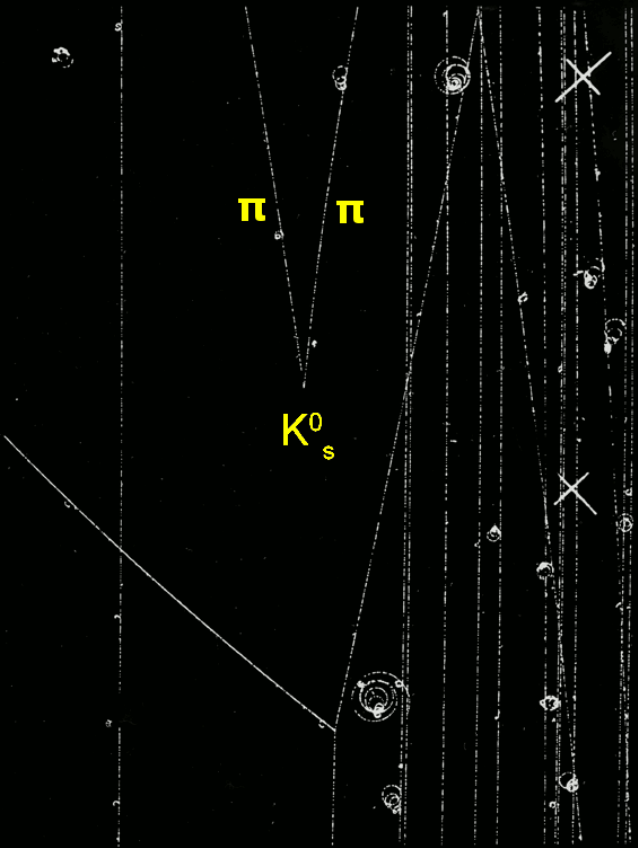
\includegraphics[height=4.2 cm]{kshort-1.png}\hspace{0.1 cm}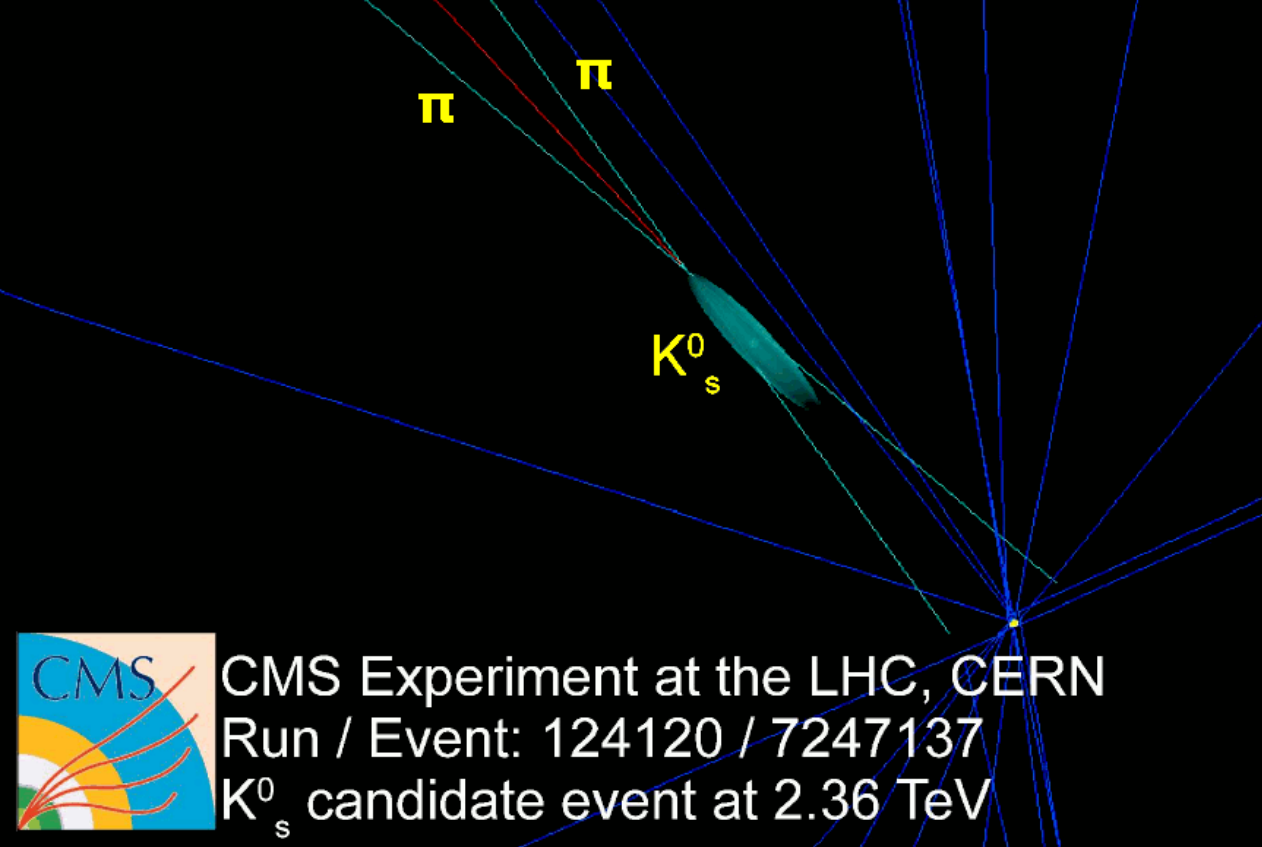
\includegraphics[height=4.2 cm]{kshort-2.png}\hspace{0.1 cm}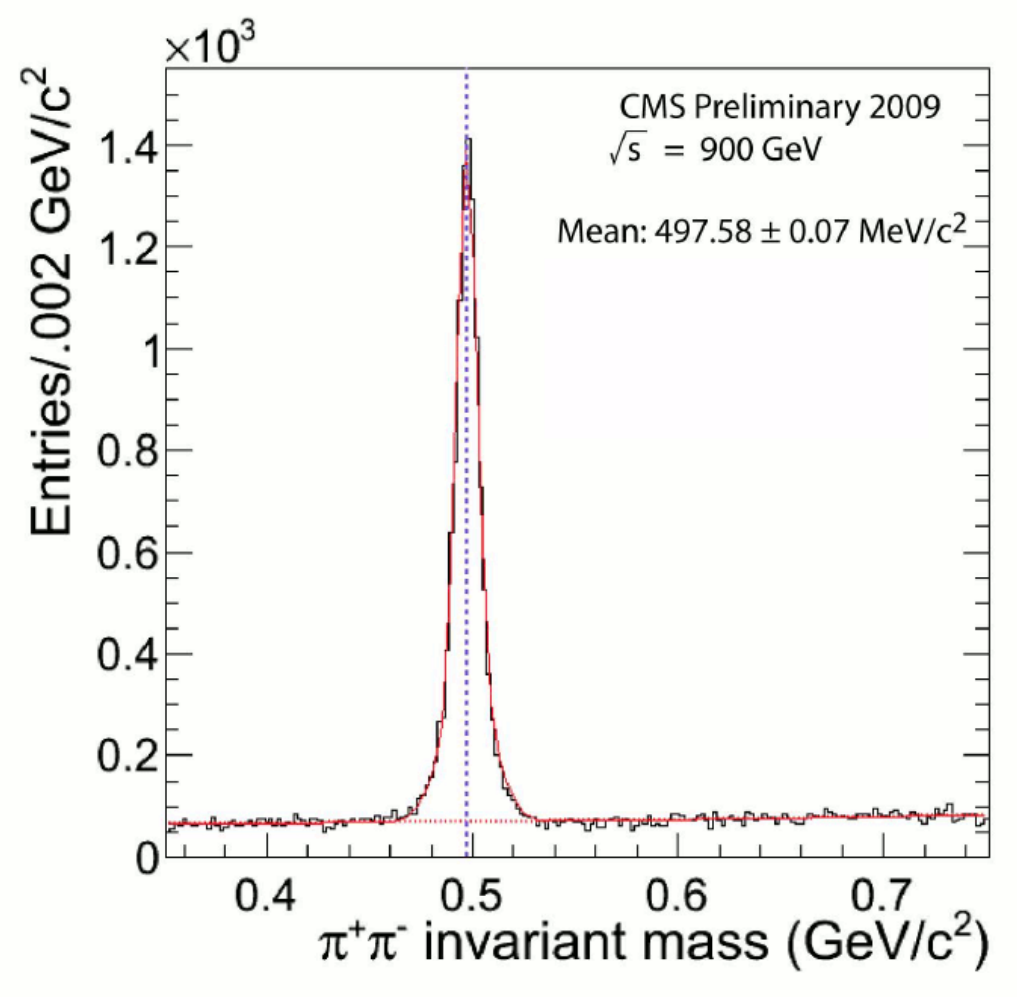
\includegraphics[height=4.2 cm]{kshort-3.png}
% \end{center}
%
% \vspace{0.15 cm}
% \begin{enumerate}
% \item Loop over all pairs of particle tracks, tentatively labeling them $\pi^+$ and $\pi^-$.
% \item Calculate m = $\sqrt{(E_{\pi^+} + E_{\pi^-})^2 - \left|\vec{p}_{\pi^+} + \vec{p}_{\pi^-}\right|^2}$.
% \item The ones with $m \sim \mbox{mass}({K_s^0}) = 0.5\mbox{ GeV}/c^2$ are good candidates.
% \end{enumerate}
% \end{frame}
%
% \begin{frame}{Apply successively down the decay chain}
% \Large
% \begin{center}
% $H \to ZZ$\hspace{1 cm}$Z \to e^+e^-$\hspace{1 cm}$Z \to \mu^+\mu^-$
% \end{center}
%
% 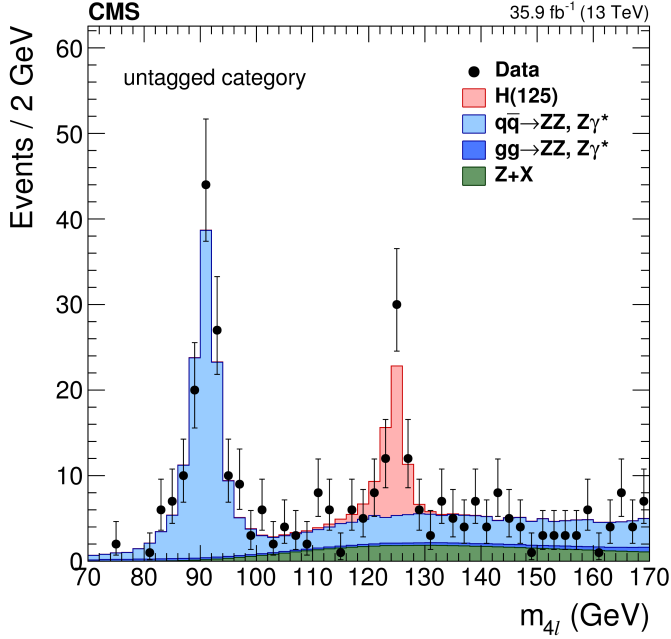
\includegraphics[height=6 cm]{higgs-to-four-leptons.png}\hfill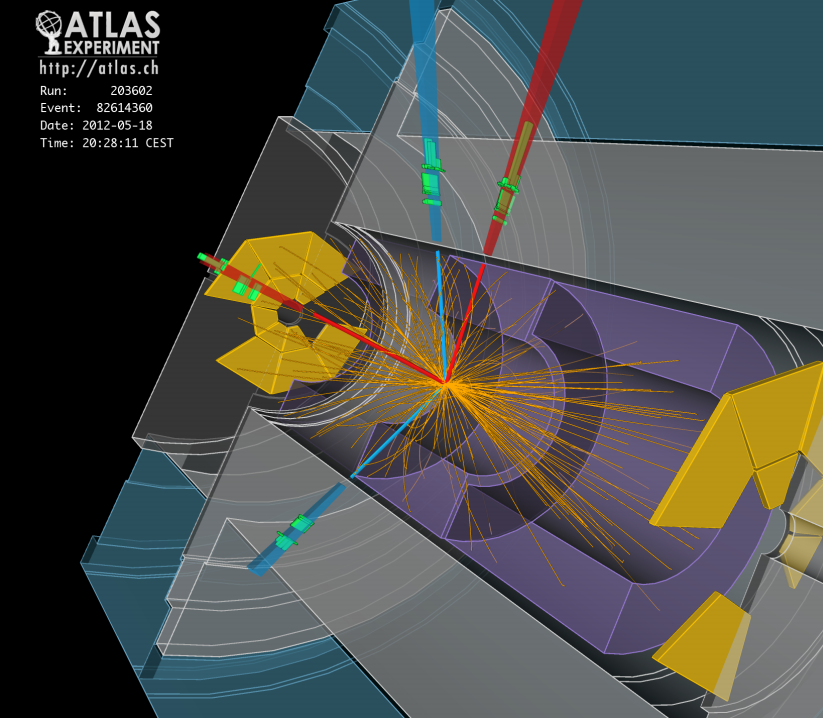
\includegraphics[height=6 cm]{higgs-to-four-leptons-2.png}
% \end{frame}

\begin{frame}{Key parts of the calculation}
\Large
\vspace{0.15 cm}
\begin{itemize}\setlength{\itemsep}{0.25 cm}
\item All events are independent; no particles or decays cross from one event to the next.
\item Detectors produce collections of different kinds of signals: tracks, energy deposition, timing\ldots
\item Candidates are generated with a \mintinline{sql}{SELF JOIN} (items from the same collection) or a \mintinline{sql}{CROSS JOIN} (items from different collections) \mintinline{sql}{ON t1.eventId == t2.eventId}.
\item Good candidates are identified by {\it filtering} (throw away bad ones) and/or {\it reduction} (pick the best of what remains.)
\end{itemize}
\end{frame}

\begin{frame}{Key parts of the calculation}
\Large
\vspace{0.5 cm}
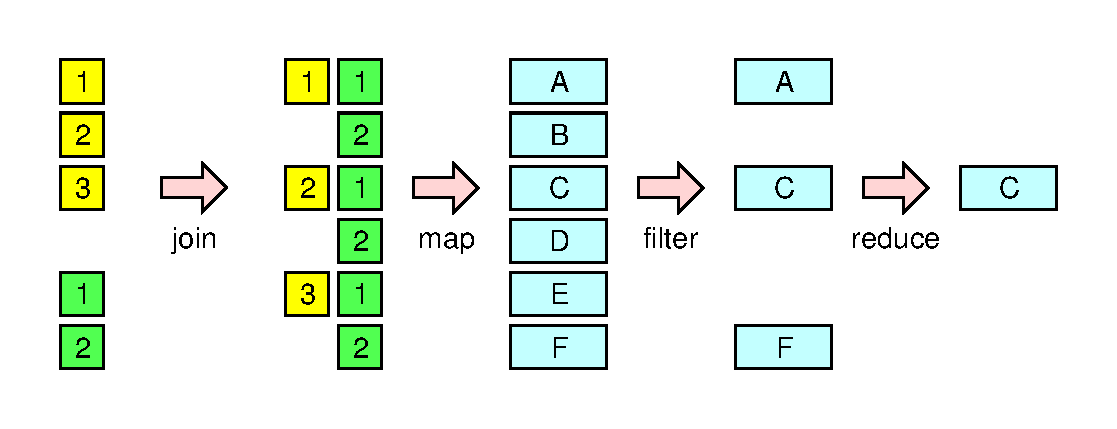
\includegraphics[width=\linewidth]{explode-flat-reduce.pdf}

\hfill \ldots independently for each event.
\end{frame}

\begin{frame}{Key part of the data structure}
\Large
\vspace{0.25 cm}
\begin{itemize}
\item Large number of events, processed in parallel.
\item Each event has an {\it arbitrary number} of record structures.
\item Not reducible to a flat table without padding and/or loss.
\end{itemize}

\vspace{0.25 cm}
\begin{columns}
\column{0.5\linewidth}
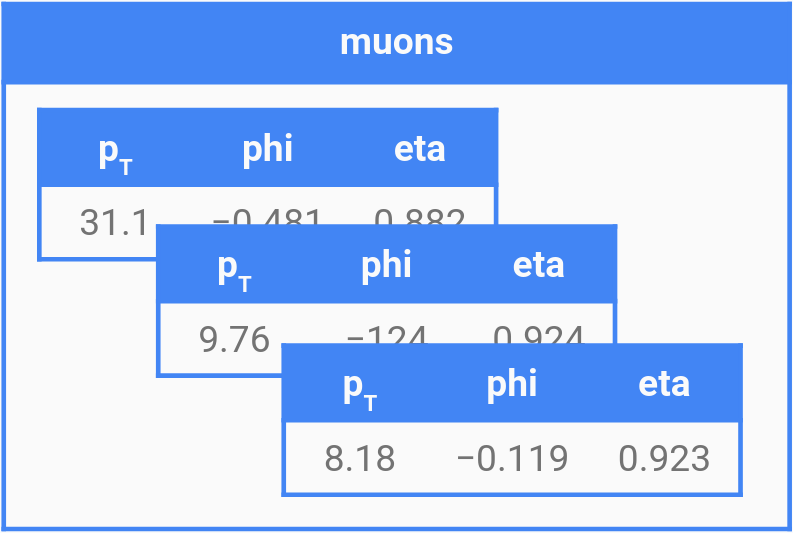
\includegraphics[width=\linewidth]{muons-as-objects.png}

\column{0.5\linewidth}
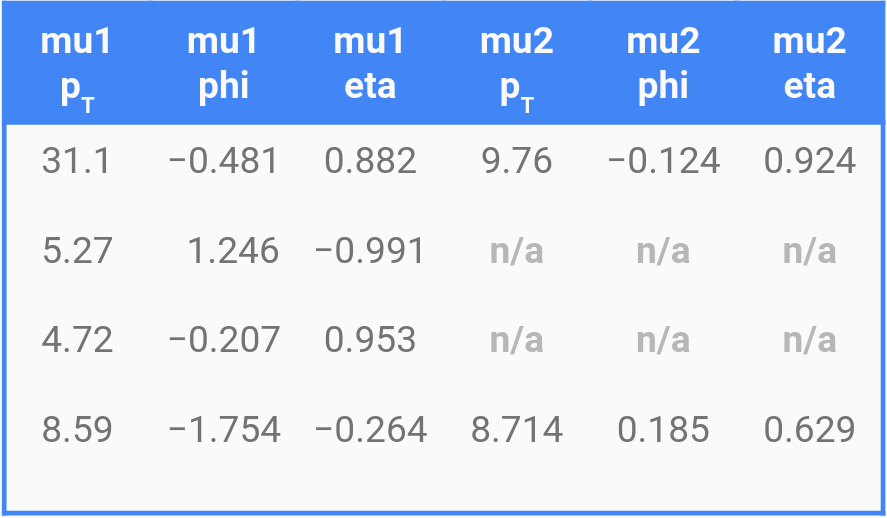
\includegraphics[width=\linewidth]{muons-as-a-table.png}
\end{columns}
\end{frame}

\begin{frame}{Programming languages used in particle physics}
\large
\vspace{0.5 cm}
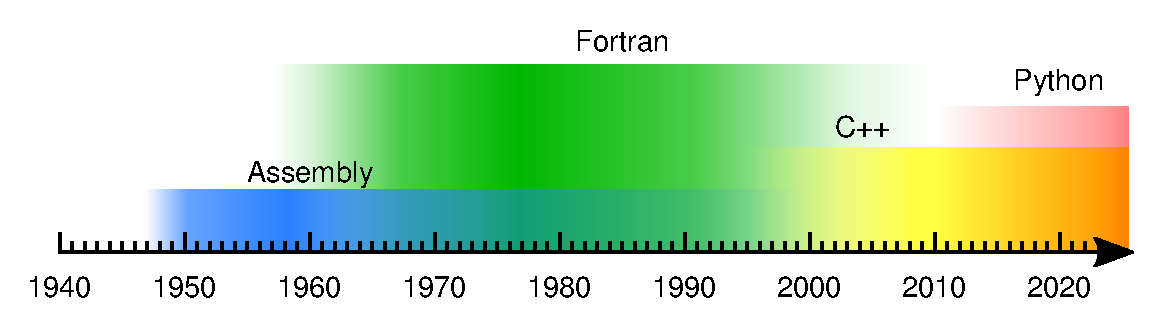
\includegraphics[width=\linewidth]{programming-languages.pdf}

\vspace{0.25 cm}
\begin{itemize}
\item First programmable computers were used for particle physics simulations.
\item Fortran was used to analyze events soon after the language was invented.
\item Major transition from Fortran to C++ in the late 1990's/early 2000's.
\item Very recent adoption of Python (alongside C++).
\end{itemize}
\end{frame}

\begin{frame}{The Python transition}
\vspace{0.2 cm}
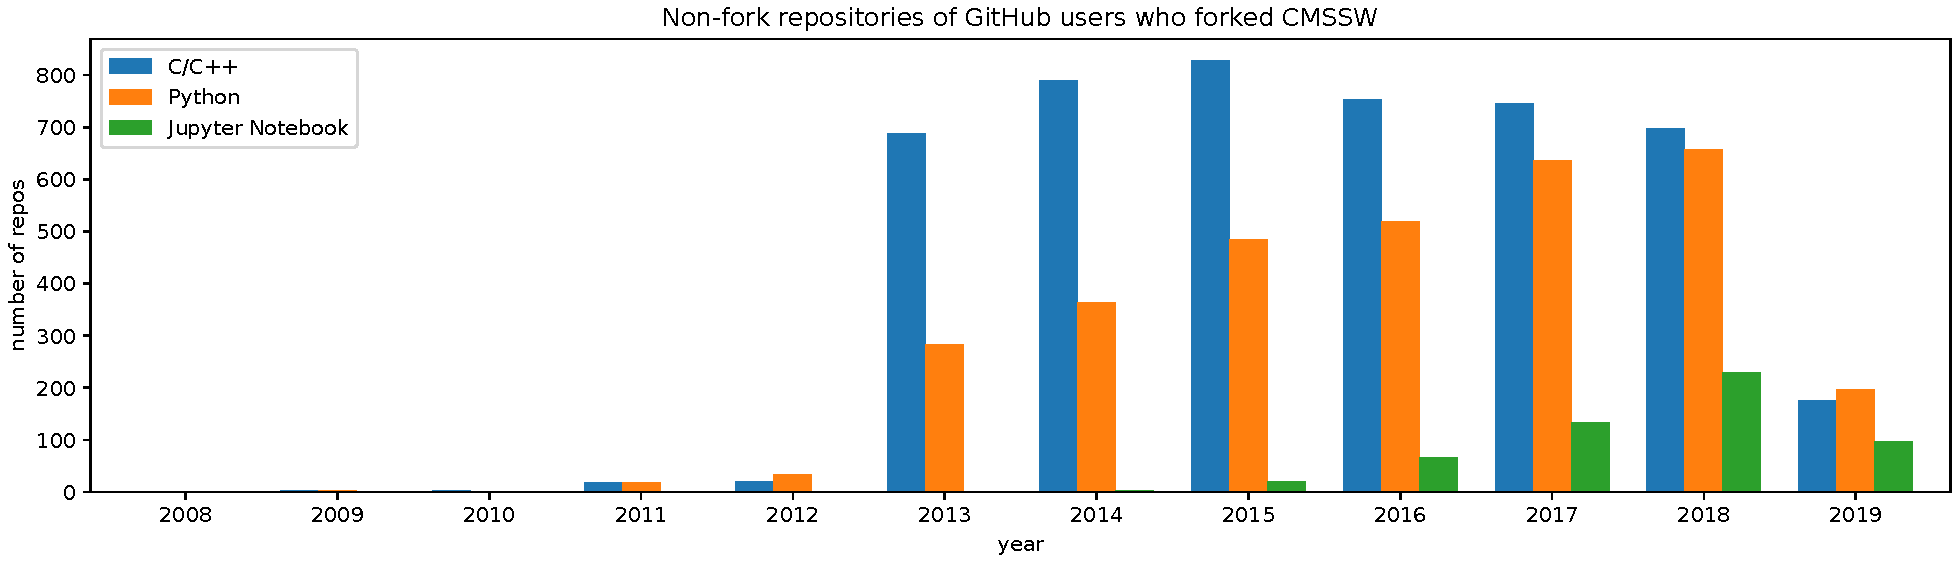
\includegraphics[width=\linewidth]{github-cmssw-lin.pdf}

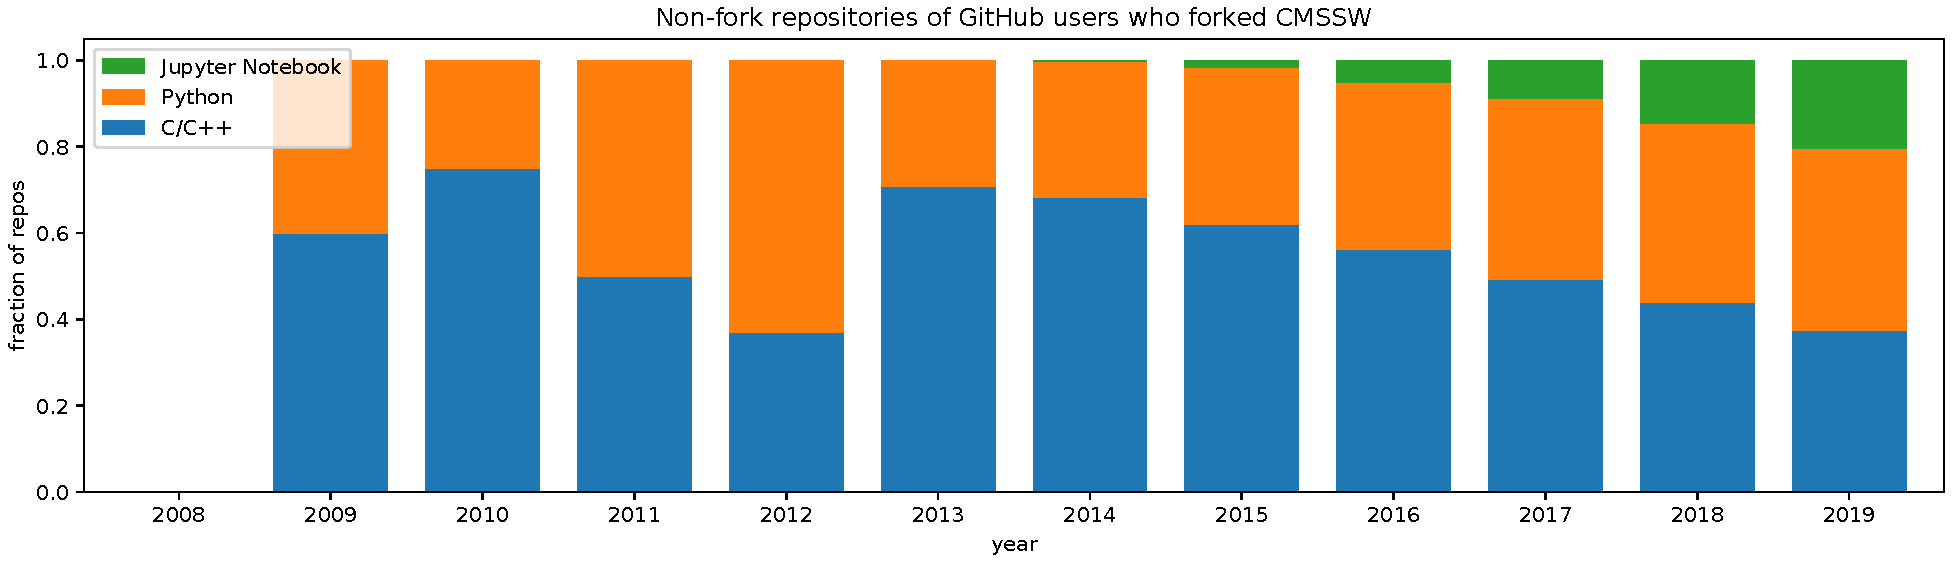
\includegraphics[width=\linewidth]{github-cmssw-frac.pdf}
\end{frame}


\begin{frame}{}
\end{frame}

\end{document}
